\documentclass[tikz, border=1mm]{standalone}
\usepackage{amsmath, amssymb}

\begin{document}
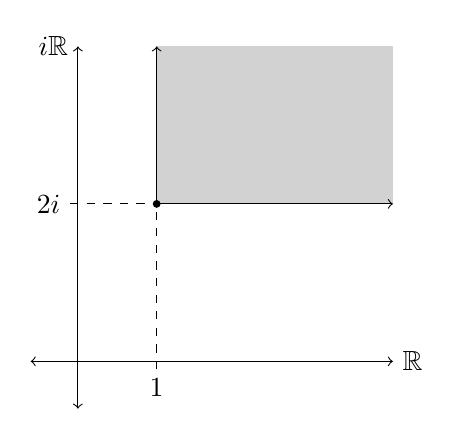
\begin{tikzpicture}[scale=1]
    \draw[<->] (-0.6, 0) -- (4, 0) node[right]{$\mathbb R$};
    \draw[<->] (0, -0.6) -- (0, 4) node[left]{$i \mathbb R$};

    \fill[gray!35] (1, 2) rectangle (4, 4);

    \draw[dashed] (-0.1, 2) node[left]{$2i$} -- (1, 2);
    \draw[dashed] (1, -0.1) node[below]{$1$} -- (1, 2);
    \draw[->] (1, 2) -- (1, 4);
    \draw[->] (1, 2) -- (4, 2);
    \draw (1, 2) node[fill, circle, inner sep=1pt]{};
\end{tikzpicture}
\end{document}
